% Sketch output, version 0.3 (build 7d, Sat Feb 9 11:09:29 2019)
% Output language: PGF/TikZ,LaTeX
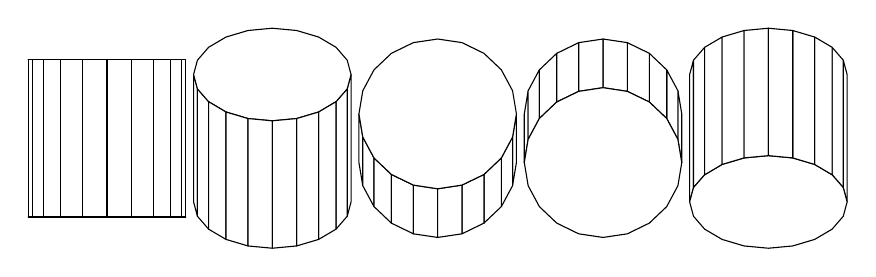
\begin{tikzpicture}[line join=round]
\filldraw[fill=white](1,-1)--(.951,-1)--(.809,-1)--(.588,-1)--(.309,-1)--(0,-1)--(-.309,-1)--(-.588,-1)--(-.809,-1)--(-.951,-1)--(-1,-1)--(-.951,-1)--(-.809,-1)--(-.588,-1)--(-.309,-1)--(0,-1)--(.309,-1)--(.588,-1)--(.809,-1)--(.951,-1)--cycle;
\filldraw[fill=white](.951,1)--(.809,1)--(.588,1)--(.309,1)--(0,1)--(-.309,1)--(-.588,1)--(-.809,1)--(-.951,1)--(-1,1)--(-.951,1)--(-.809,1)--(-.588,1)--(-.309,1)--(0,1)--(.309,1)--(.588,1)--(.809,1)--(.951,1)--(1,1)--cycle;
\filldraw[fill=white](3.249,-.603)--(3.249,.015)--(3.2,.309)--(3.2,-.309)--cycle;
\filldraw[fill=white](5.2,-.309)--(5.2,.309)--(5.151,.015)--(5.151,-.603)--cycle;
\filldraw[fill=white](7.251,.603)--(7.251,-.015)--(7.3,-.309)--(7.3,.309)--cycle;
\filldraw[fill=white](5.3,.309)--(5.3,-.309)--(5.349,-.015)--(5.349,.603)--cycle;
\filldraw[fill=white](3.391,-.868)--(3.391,-.25)--(3.249,.015)--(3.249,-.603)--cycle;
\filldraw[fill=white](7.109,.868)--(7.109,.25)--(7.251,-.015)--(7.251,.603)--cycle;
\filldraw[fill=white](5.151,-.603)--(5.151,.015)--(5.009,-.25)--(5.009,-.868)--cycle;
\filldraw[fill=white](5.349,.603)--(5.349,-.015)--(5.491,.25)--(5.491,.868)--cycle;
\filldraw[fill=white](3.612,-1.078)--(3.612,-.46)--(3.391,-.25)--(3.391,-.868)--cycle;
\filldraw[fill=white](6.888,1.078)--(6.888,.46)--(7.109,.25)--(7.109,.868)--cycle;
\filldraw[fill=white](5.491,.868)--(5.491,.25)--(5.712,.46)--(5.712,1.078)--cycle;
\filldraw[fill=white](5.009,-.868)--(5.009,-.25)--(4.788,-.46)--(4.788,-1.078)--cycle;
\filldraw[fill=white](3.891,-1.214)--(3.891,-.595)--(3.612,-.46)--(3.612,-1.078)--cycle;
\filldraw[fill=white](6.609,1.214)--(6.609,.595)--(6.888,.46)--(6.888,1.078)--cycle;
\filldraw[fill=white](4.788,-1.078)--(4.788,-.46)--(4.509,-.595)--(4.509,-1.214)--cycle;
\filldraw[fill=white](5.712,1.078)--(5.712,.46)--(5.991,.595)--(5.991,1.214)--cycle;
\filldraw[fill=white](4.2,-1.26)--(4.2,-.642)--(3.891,-.595)--(3.891,-1.214)--cycle;
\filldraw[fill=white](4.509,-1.214)--(4.509,-.595)--(4.2,-.642)--(4.2,-1.26)--cycle;
\filldraw[fill=white](6.3,1.26)--(6.3,.642)--(6.609,.595)--(6.609,1.214)--cycle;
\filldraw[fill=white](5.991,1.214)--(5.991,.595)--(6.3,.642)--(6.3,1.26)--cycle;
\filldraw[fill=white](1.149,-.991)--(1.149,.627)--(1.1,.809)--(1.1,-.809)--cycle;
\filldraw[fill=white](3.1,-.809)--(3.1,.809)--(3.051,.627)--(3.051,-.991)--cycle;
\filldraw[fill=white](9.351,.991)--(9.351,-.627)--(9.4,-.809)--(9.4,.809)--cycle;
\filldraw[fill=white](7.4,.809)--(7.4,-.809)--(7.449,-.627)--(7.449,.991)--cycle;
\filldraw[fill=white](1.291,-1.155)--(1.291,.464)--(1.149,.627)--(1.149,-.991)--cycle;
\filldraw[fill=white](9.209,1.155)--(9.209,-.464)--(9.351,-.627)--(9.351,.991)--cycle;
\filldraw[fill=white](7.449,.991)--(7.449,-.627)--(7.591,-.464)--(7.591,1.155)--cycle;
\filldraw[fill=white](3.051,-.991)--(3.051,.627)--(2.909,.464)--(2.909,-1.155)--cycle;
\filldraw[fill=white](3.051,.991)--(2.909,1.155)--(2.688,1.285)--(2.409,1.368)--(2.1,1.397)--(1.791,1.368)--(1.512,1.285)--(1.291,1.155)--(1.149,.991)--(1.1,.809)--(1.149,.627)--(1.291,.464)--(1.512,.333)--(1.791,.25)--(2.1,.221)--(2.409,.25)--(2.688,.333)--(2.909,.464)--(3.051,.627)--(3.1,.809)--cycle;
\filldraw[fill=white](9.351,-.627)--(9.209,-.464)--(8.988,-.333)--(8.709,-.25)--(8.4,-.221)--(8.091,-.25)--(7.812,-.333)--(7.591,-.464)--(7.449,-.627)--(7.4,-.809)--(7.449,-.991)--(7.591,-1.155)--(7.812,-1.285)--(8.091,-1.368)--(8.4,-1.397)--(8.709,-1.368)--(8.988,-1.285)--(9.209,-1.155)--(9.351,-.991)--(9.4,-.809)--cycle;
\filldraw[fill=white](1.512,-1.285)--(1.512,.333)--(1.291,.464)--(1.291,-1.155)--cycle;
\filldraw[fill=white](8.988,1.285)--(8.988,-.333)--(9.209,-.464)--(9.209,1.155)--cycle;
\filldraw[fill=white](7.591,1.155)--(7.591,-.464)--(7.812,-.333)--(7.812,1.285)--cycle;
\filldraw[fill=white](2.909,-1.155)--(2.909,.464)--(2.688,.333)--(2.688,-1.285)--cycle;
\filldraw[fill=white](-.951,-1)--(-.951,1)--(-1,1)--(-1,-1)--cycle;
\filldraw[fill=white](1,-1)--(1,1)--(.951,1)--(.951,-1)--cycle;
\filldraw[fill=white](1.791,-1.368)--(1.791,.25)--(1.512,.333)--(1.512,-1.285)--cycle;
\filldraw[fill=white](2.688,-1.285)--(2.688,.333)--(2.409,.25)--(2.409,-1.368)--cycle;
\filldraw[fill=white](8.709,1.368)--(8.709,-.25)--(8.988,-.333)--(8.988,1.285)--cycle;
\filldraw[fill=white](7.812,1.285)--(7.812,-.333)--(8.091,-.25)--(8.091,1.368)--cycle;
\filldraw[fill=white](2.1,-1.397)--(2.1,.221)--(1.791,.25)--(1.791,-1.368)--cycle;
\filldraw[fill=white](2.409,-1.368)--(2.409,.25)--(2.1,.221)--(2.1,-1.397)--cycle;
\filldraw[fill=white](8.091,1.368)--(8.091,-.25)--(8.4,-.221)--(8.4,1.397)--cycle;
\filldraw[fill=white](8.4,1.397)--(8.4,-.221)--(8.709,-.25)--(8.709,1.368)--cycle;
\filldraw[fill=white](-.809,-1)--(-.809,1)--(-.951,1)--(-.951,-1)--cycle;
\filldraw[fill=white](.951,-1)--(.951,1)--(.809,1)--(.809,-1)--cycle;
\filldraw[fill=white](-.588,-1)--(-.588,1)--(-.809,1)--(-.809,-1)--cycle;
\filldraw[fill=white](.809,-1)--(.809,1)--(.588,1)--(.588,-1)--cycle;
\filldraw[fill=white](5.151,.603)--(5.009,.868)--(4.788,1.078)--(4.509,1.214)--(4.2,1.26)--(3.891,1.214)--(3.612,1.078)--(3.391,.868)--(3.249,.603)--(3.2,.309)--(3.249,.015)--(3.391,-.25)--(3.612,-.46)--(3.891,-.595)--(4.2,-.642)--(4.509,-.595)--(4.788,-.46)--(5.009,-.25)--(5.151,.015)--(5.2,.309)--cycle;
\filldraw[fill=white](7.251,-.015)--(7.109,.25)--(6.888,.46)--(6.609,.595)--(6.3,.642)--(5.991,.595)--(5.712,.46)--(5.491,.25)--(5.349,-.015)--(5.3,-.309)--(5.349,-.603)--(5.491,-.868)--(5.712,-1.078)--(5.991,-1.214)--(6.3,-1.26)--(6.609,-1.214)--(6.888,-1.078)--(7.109,-.868)--(7.251,-.603)--(7.3,-.309)--cycle;
\filldraw[fill=white](-.309,-1)--(-.309,1)--(-.588,1)--(-.588,-1)--cycle;
\filldraw[fill=white](.588,-1)--(.588,1)--(.309,1)--(.309,-1)--cycle;
\filldraw[fill=white](0,-1)--(0,1)--(-.309,1)--(-.309,-1)--cycle;
\filldraw[fill=white](.309,-1)--(.309,1)--(0,1)--(0,-1)--cycle;
\end{tikzpicture}% End sketch output
